%%% template.tex
%%%
%%% This LaTeX source document can be used as the basis for your technical
%%% paper or abstract. Intentionally stripped of annotation, the parameters
%%% and commands should be adjusted for your particular paper - title, 
%%% author, article DOI, etc.
%%% The accompanying ``template.annotated.tex'' provides copious annotation
%%% for the commands and parameters found in the source document. (The code
%%% is identical in ``template.tex'' and ``template.annotated.tex.'')

\documentclass[conference, 12pt]{acmsiggraph}

\title{Rotation Averaging for Global SfM}

\author{Bryce Evans \and Rafael Farias Marinheiro}
% \contactemail{}
\affiliation{Cornell University\thanks{\{bae43, rf356\}@cornell.edu}}
\pdfauthor{Rafael F. Marinheiro}

\keywords{crowd simulation, user interaction, real-time rendering}

\usepackage{amsmath}
\usepackage{amssymb}
\usepackage{subcaption}
\usepackage{algorithm}
\usepackage{algpseudocode}
% \usepackage{algorithm}

\begin{document}

%% \teaser{
%%   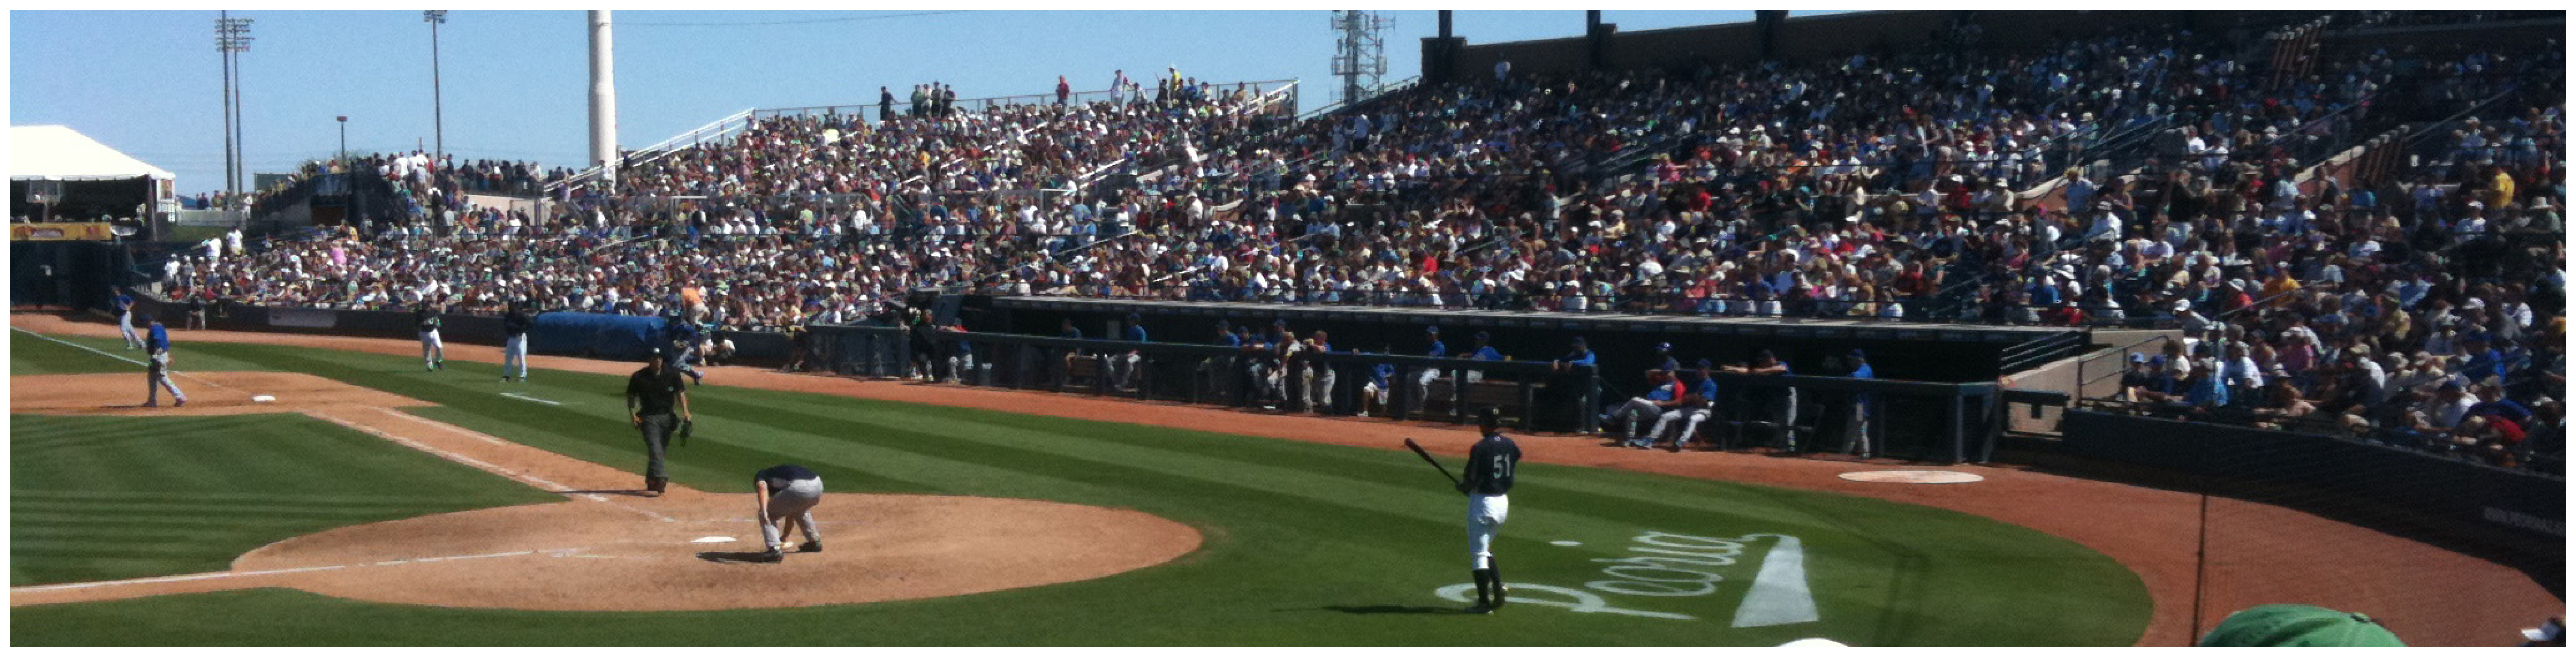
\includegraphics[height=1.5in]{images/sampleteaser}
%%   \caption{Spring Training 2009, Peoria, AZ.}
%% }

\maketitle

% \begin{abstract}

% We intend to create a interactive Crowd Simulation application using the approach described in \cite{kim2012interactive}. The user will be able to interact with the application with a commodity depth sensor \cite{Zhang:2012:MKS:2225053.2225203}, modifying the environment in real time.

% \end{abstract}

% \begin{figure}[Ht!]
%   \centering
%     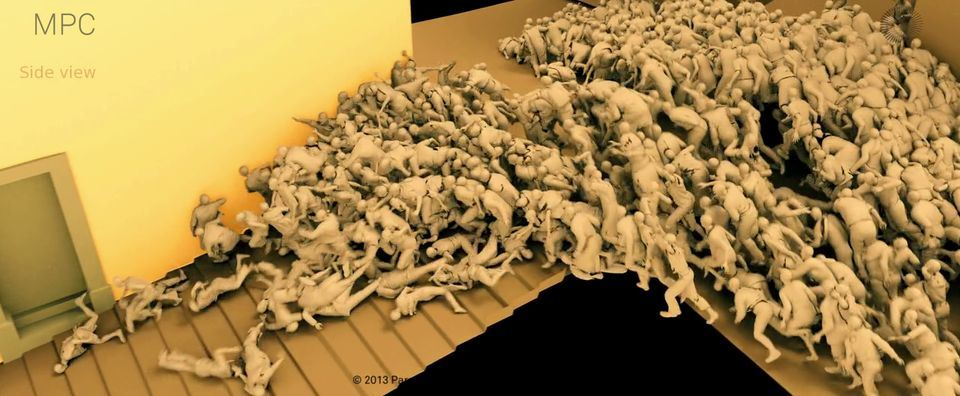
\includegraphics[width=0.5\textwidth]{images/mpc3.jpg}
%     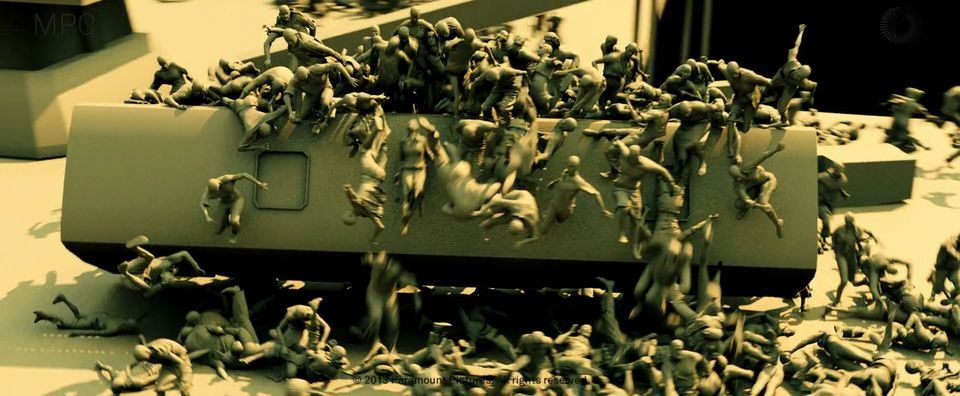
\includegraphics[width=0.5\textwidth]{images/mpc2.jpg}
% 	\caption{World War Z (2013). Zombie agents were computationally simulated.}
% 	\label{fig:wwz}
% \end{figure}

% %% Use this only if you're preparing a technical paper to be published in the 
% %% ACM 'Transactions on Graphics' journal.

% \begin{CRcatlist}
% 	\CRcat{I.2.11}{Artificial Intelligence}{Distributed Artificial Intelligence}{Multiagent systems};
% 	\CRcat{I.3.7}{Computer Graphics}{Three-Dimensional Graphics and Realism}{Animation};
% 	\CRcat{I.6.8}{Simulation and Modeling}{Types of Simulation}{Animation}
% \end{CRcatlist}

% %%% The ``\keywordlist'' prints out the user-defined keywords.

% \keywordlist

% \TOGlinkslist

% %% Required for all content. 

% \copyrightspace

\section{Introduction}

Structure from motion is a powerful tool in reconstructing environments without artist modeling. By taking a series of images and finding common points between them, a network of relative camera is created to represent the scene but often has error that causes the reconstruction to have no feasible solution. Robust and efficient rotation averaging \cite{rotation} proposes several methods to solve this problem, but does not provide well useable code. Given the power in SfM applications, there is a long pipeline of steps but they are fractured and inconsistent. We present a Python module publicly available to integrate into the greater pipeline that solves the rotation averaging problem and interfaces well with other code available such as the translation averaging solver by \cite{translation}.

\section{Background}

Current SfM pipelines can be divided in two different classes: An Iterative SfM pipeline (see figure \ref{fig:iterative}) will try to iteratively add cameras to the working set and it will run a bundle adjustment after each iteration. The quality of the results generated by such pipelines depends on the ordering of the cameras and it is highly sensitive to outliers. One example of such a pipeline is the well-known PhotoTourism \cite{snavely2006photo}.

An Global SfM pipeline (see figure \ref{fig:global}) will instead divide the problem in two different global subproblems: The Rotation Averaging problem and the Translation Averaging problem. These problems can be described as follows: Consider a connected graph $G = (V,E)$. Associated with each edge $e = (i, j)$, there is a relative rotation $R_{ij} \in SO(3)$ and relative translation $t_{ij} \in R^3$. We want to assign to each vertex of the graph a global rotation and translation $R_i, t_i$ such that we minimize:

\begin{eqnarray}
	\sum_{(i,j) \in E} d_1(R_{j}R_{i}^{-1}, R_{ij}) \\
	\sum_{(i,j) \in E} d_2(t_{j}-t_{i}, R_{i}t_{ij})
\end{eqnarray}

Where $d_1$ and $d_2$ are metrics of $SO(3)$ and $R^3$ respectively. The first equation describes the Rotation Averaging Problem and the second equation describes the Translation Averaging problem. Both problems can be solved globally, so the final solution does not depend on the ordering of the cameras and it is more robust when working with outliers.

In this project, we have implemented the approach described in \cite{rotation} to solve the Rotation Averaging problem and we have used the approach described in \cite{translation} to solve the Translation Averaging problem. 

\begin{figure}[H]
  \centering
  \begin{subfigure}{0.5\textwidth}
  	\centering
    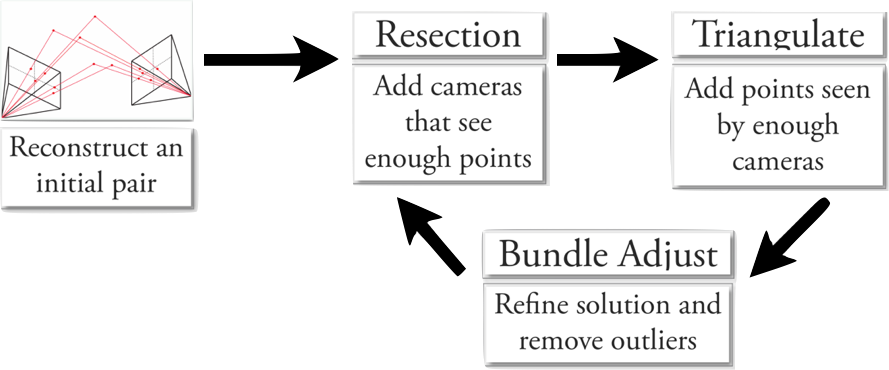
\includegraphics[width=1.0\textwidth]{images/iterative_sfm.png}
	\caption{Iterative SfM Pipeline}
	\label{fig:iterative}
  \end{subfigure}

  \begin{subfigure}{0.5\textwidth}
  	\centering
    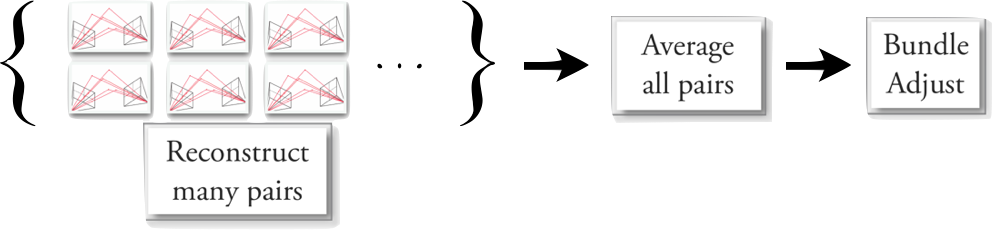
\includegraphics[width=1.0\textwidth]{images/global_sfm.png}
	\caption{Global SfM Pipeline}
	\label{fig:global}
  \end{subfigure}
  \caption{(a) On top, the Iterative SfM Pipeline. (b) At bottom, the Global SfM Pipeline.}
  \label{fig:pipelines}
\end{figure}

\section{Rotation Averaging}

A Rotation Matrix $R$ is a $3 \times 3$ orthonormal matrix (i.e., $RR^\intercal = I = R^\intercal R$) such that $|R| = +1$. All rotation matrices form a closed group known as the Special Orthonormal Group $SO(3)$. The $SO(3)$ is also a Lie Group, so it has the following properties: (1) The neighborhood of a point in the group is topologically equivalent to a vector space known as the Lie algebra. (2) There exist a direct mapping between an element in the Lie Group and an element in the Lie Algebra. In the case of $SO(3)$, the associated Lie Algebra is know as $\mathfrak{so}(3)$.

The first property can be used to locally linearize the Rotation Averaging problem. Let $\omega = \theta n \in \mathfrak{so}(3)$, be the vector in the Lie Algebra that represents the rotation by $\theta$ radians around the unit-norm axis $n$. Let $R \in SO(3)$ be the equivalent rotation matrix (i.e. $\omega = \log(R)$). We can extrapolate the properties of the Lie Group to use the following approximation: 

\begin{equation}
\log(R_{j}R_{i}^{-1}) = \log(R_{ij}) = \omega_{ij} \approx \omega_{j} - \omega_{i}
\label{eqn:approx_lie}
\end{equation}

Given the set of relative rotations, one can write a matrix $A$ that encodes a linear system with all the equation involving $\omega_{ij}$. Then, we would have the following linear system:

\begin{equation}
A\omega_{global} = \omega_{rel}
\end{equation}

However, equation (\ref{eqn:approx_lie}) is an approximation. So instead of solving directly for $\omega_{global}$, we can iteratively compute the error of our solution ($\Delta\omega_{rel}$) and then we can update our solution ($\Delta\omega_{global}$) by using the following equation:
\begin{equation}
A\Delta\omega_{global} = \Delta\omega_{rel}
\end{equation}

The algorithm is described in listings (\ref{algo:rot}). The linear system in line (\ref{algo:rot}:\ref{algo:roteq}) can be solved using different methods. One could use the Linear Least Squares Method to solve it, however it is not robust enough to deal with outliers. Instead, we use two different methods. The first one ($\ell1$ Rotation Averaging - $\ell1$RA) tries to minimize the $\ell1$-norm, i.e., it tries to minimize $|Ax - b|_1$ and the second one (Iteratively Reweighted Least Squares - IRLS) tries to robustly minimize the $\ell2$-norm (See \cite{rotation} for more details).

\begin{algorithm}[h]
  \caption{Rotation Averaging Algorithm}\label{algo:rot}
  \begin{algorithmic}[1]
    \State \textbf{Input:} The Relative Rotations $R_{rel} = \{R_{ij}\}$ and an initial guess of the solution
    \State \textbf{Output:} The Global Rotations $R_{global} = \{R_{i}\}$ 
    \Procedure{RotationAveraging}{$R_{rel}$, $R_{guess}$}
    \State $A \gets ComputeMatrix(R_{rel})$
    \ForAll{$(i, j) \in R_{rel}$} \Comment{Compute $\Delta\omega_{rel}$}
    \State $\Delta R_{ij} \gets R_{j}^{-1}R_{ij}R_{i}$
    \State $\Delta\omega_{ij} \gets \log(\Delta R_{ij})$
    \EndFor
    \While{$|\Delta\omega_{rel}| \ge \epsilon$}
    	\State $\Delta\omega_{global} \gets A\backslash \Delta\omega_{rel}$ \Comment{Solve for $\Delta\omega_{global}$} \label{algo:roteq}
    	\ForAll{$i\in R_{global}$} \Comment{Update the solution}
	    \State $R_{i} \gets R_{i}\exp(\Delta\omega_{i})$
	    \EndFor
    \EndWhile
    \State \textbf{return} $R_{global}$
    \EndProcedure
  \end{algorithmic}
\end{algorithm}

\section{Implementation and Results}

We have implemented the Rotation Averaging algorithms in Python. The source code only depends on a few Python packages (SciPy \cite{scipy} and NetworkX \cite{networkx}) and it is publicly available\footnote{\url{https://github.com/RafaelMarinheiro/RotationAveraging}}. We have also integrated our implementation with the SfM Init package\footnote{\url{https://github.com/RafaelMarinheiro/SfMInit}} \cite{translation}.

An initial guess for the Global Rotations is required to use these algorithms. To find the initial guess, we proceed as follows: Given the graph $G = (V, E)$, we assign to each edge $(i, j)$ a weight $w(i, j) = d(R_{ij}, I)$, then we choose the edges of the Minimum Spanning Tree. Then, we select a random camera and we assign the Global Rotation for each vertex using a Depth-First Order approach.

In our implementation, we have discovered that the algorithm has some numerical problems. For instance, if the input matrices are not quite rotation matrices, the conversions between $SO(3)$ and $\mathfrak{so}(3)$ and vice-versa will fail drastically. To solve this problem, we find the closest orthonormal matrix to the input matrix using the formula: $O = M(M^\intercal M)^{-\frac{1}{2}}$. 

\begin{figure}[H]
  \centering
  \begin{subfigure}{0.5\textwidth}
    \centering
    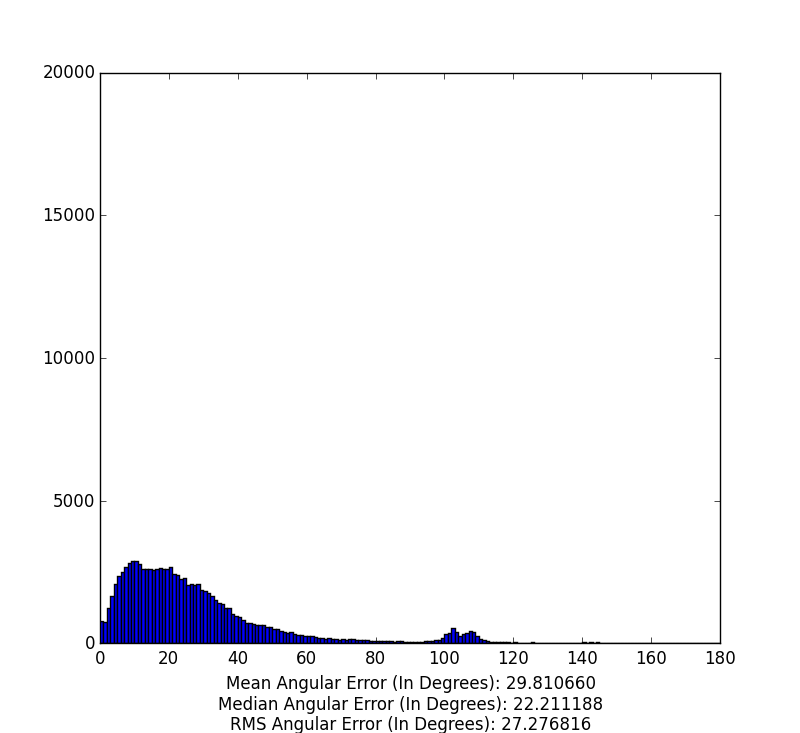
\includegraphics[width=0.81\textwidth]{images/final_span.png}
    \caption{Initial guess after Spanning Tree}
    \label{fig:post_span}
  \end{subfigure}

    \begin{subfigure}{0.5\textwidth}
    \centering
    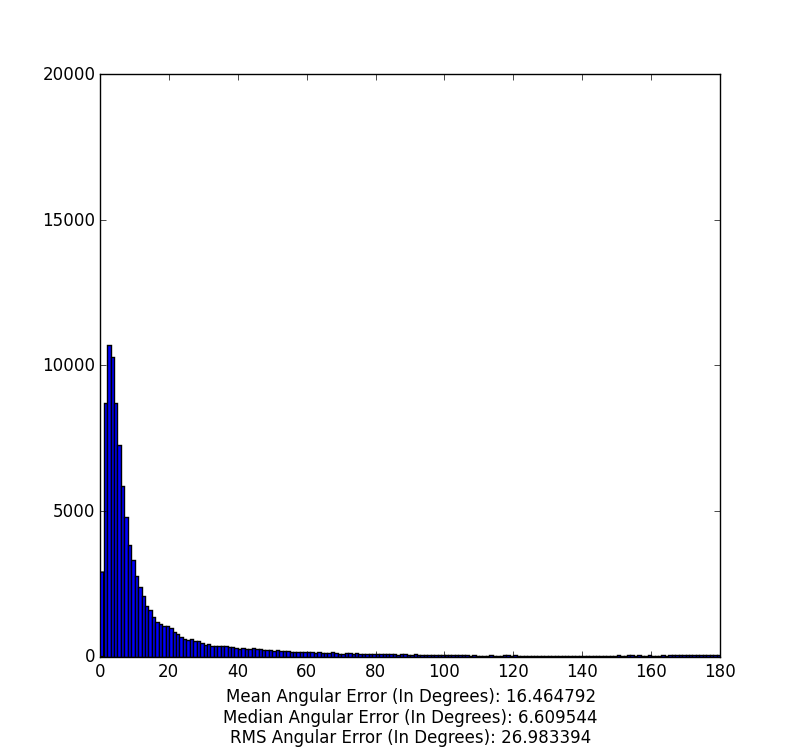
\includegraphics[width=0.81\textwidth]{images/final_post_l1.png}
    \caption{After $\ell1$RA}
    \label{fig:post_l1ra}
  \end{subfigure}

    \begin{subfigure}{0.5\textwidth}
    \centering
    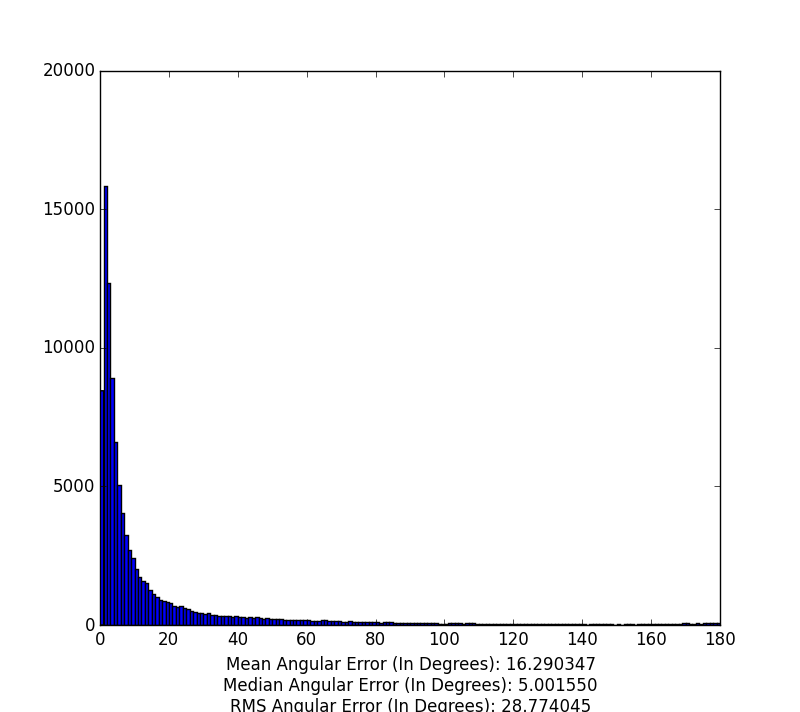
\includegraphics[width=0.81\textwidth]{images/final_post_irls.png}
    \caption{After IRLS}
    \label{fig:post_irls}
  \end{subfigure}

  \caption{Histogram of error after each part of the algorithm. The abscissa value represents the error in degrees. The closer to zero, the better.}
  \label{fig:results}
\end{figure}

We have tested our implementation against the Notredame dataset published by \cite{translation}. Figure (\ref{fig:results}) shows the error after each step of the algorithm. First, we run the Spanning Tree algorithm described earlier (see figure \ref{fig:post_span}), then we run only 5 iterations of the $\ell1$RA algorithm (see figure \ref{fig:post_l1ra}). After that, we use the output of the $\ell1$RA algorithm as an input to the IRLS algorithm and then we run 20 iterations of it (see figure \ref{fig:post_irls}). Notice that the error is indeed reduced after each step. The reported error metrics do match the results published both by \cite{rotation} and \cite{translation}.

\section{Conclusion}

In summary, we have successfuly implemented a Rotation Averaging algorithm. We have also made the code publicly available. Our implementation is easily extensible and it does not depend on non-free tools, so we hope that this will be a valuable tool for the research community.

\bibliographystyle{acmsiggraph}
\bibliography{proposal}

\end{document}
